\documentclass[12pt]{article}
\usepackage{xcolor, colortbl}
\usepackage{algorithm}
\usepackage[noend]{algpseudocode}
\usepackage{textcomp}
\usepackage{listings}
\usepackage{hyperref}
\usepackage{alltt}
\usepackage{tikz}
\usepackage{framed}
\usepackage{mdframed}
\usepackage{marvosym}
\usepackage{wasysym}
\usepackage{marvosym}
\usepackage{crayola}
\usepackage{mathpartir}
\usepackage{tabularx}
\usepackage[belowskip=-15pt,aboveskip=0pt]{caption}
\usepackage[skins]{tcolorbox}
\usepackage{multicol}
\usetikzlibrary{positioning,shapes,arrows, backgrounds, fit, shadows}
\usetikzlibrary{decorations.markings}
\usepackage{listings}
\usepackage[margin=1in]{geometry}
\usepackage{mathptmx}
\usepackage{setspace}
\usepackage{natbib}
\usepackage{authblk}

\newcommand{\myheader}[1]{
	{\color{darkblue}
		\begin{Large}
			\begin{center}
				{#1}
			\end{center}
		\end{Large}
	}
}
\newcommand{\myminorheader}[1]{
	{\color{BrickRed}
		\begin{Large}
			{\fontfamily{\sfdefault}\selectfont\textbf{#1}}
		\end{Large}
	}
}

%\tikzstyle{input} = [coordinate]
%\tikzstyle{output} = [coordinate]


\tikzstyle{bb}=[%
      rectangle, draw=black, thick, fill=OliveGreen!30, drop shadow, align=center,
      text ragged, minimum height=2em, minimum width=2em, inner sep=6pt
]

\tikzstyle{inv}=[%
      rectangle, draw=none,  align=center,
      text ragged, minimum height=2em, minimum width=2em, inner sep=6pt
]

\tikzstyle{db}=[%
      ellipse, draw=black, thick, fill=pink, drop shadow, align=center,
      text ragged, minimum height=2em, inner sep=6pt
]

\tikzstyle{jn}=[%
      ellipse, draw=black, thick, fill=black
]

\tikzstyle{io}=[%
      trapezium, trapezium left angle=60, trapezium right angle=120, draw=black, thick, fill=brown, drop shadow,
      text ragged, minimum height=2em, minimum width=2em, inner sep=6pt, align=center
]

\tikzstyle{glio}=[%
      trapezium, trapezium left angle=60, trapezium right angle=120, draw=red, line width = 1mm, fill=brown, drop shadow,
      text ragged, minimum height=2em, minimum width=2em, inner sep=6pt
]
\tikzstyle{gl}=[%
      rectangle, draw=red, line width = 1mm, fill=lightblue, drop shadow,
      text ragged, minimum height=2em, minimum width=2em, inner sep=6pt
]

\tikzstyle{en}=[%
      rectangle, draw=black, thick, fill=none,
      text ragged, minimum height=2em, minimum width=2em, inner sep=6pt
]

\tikzstyle{sh}=[%
      rectangle, draw=gray, thick, fill=none, color = gray,
      text ragged, minimum height=2em, minimum width=2em, inner sep=6pt
]


\lstdefinestyle{pc}{
	language = Python,
	basicstyle = \small\ttfamily,
	stringstyle = \ttfamily\color{Purple},
	keywordstyle=\color{black}\bfseries,
	identifierstyle=\ttfamily\color{BrickRed},
	frame=single,
	frameround=tttt,
	numbers=none,
	showstringspaces=false
}

\lstdefinestyle{jc}{
	language = Java,
	basicstyle = \normal\ttfamily,
	stringstyle = \ttfamily,
	keywordstyle=\color{Blue}\bfseries,
	identifierstyle=\color{Pink},
	commentstyle=\color{darkgreen},
	frame=single,
	frameround=tttt,
	showstringspaces=false
}

\lstdefinestyle{occ}{
	language = Caml,
	basicstyle = \ttfamily,
	stringstyle = \color{red}\ttfamily,
	keywordstyle=\color{Blue}\bfseries,
	identifierstyle=\ttfamily,
	frameround=tttt,
	numbers=none,
	showstringspaces=false,
	escapeinside={(*@}{@*)}
}

\lstdefinestyle{oc}{
	language = bash,
	backgroundcolor = \color{black!60},
	basicstyle = \ttfamily\color{white},
	stringstyle = \color{red}\ttfamily,
	keywordstyle=\color{white}\bfseries,
	identifierstyle=\ttfamily,
	frameround=tttt,
	numbers=none,
	showstringspaces=false,
	escapeinside={(*@}{@*)}
}

\doublespacing

\title{Automated Evaluation of Programming Assignments -- An Experience Report}
\author[]{Sujit Kumar Chakrabarti \\ \texttt{sujitkc@iiitb.ac.in}}
\affil[]{
International Institute of Information Technology -- Bangalore \\
26/C, Electronics City Ph-1 \\
Hosur Road, Bangalore-560100 \\
Ph.: \texttt{+91 80 4140 7777} \\
Fax: \texttt{+91 80 4140 7704}  
}
\date{}

\titlepage
\begin{document}
\maketitle
\begin{titlepage}
\title{Automated Evaluation of Programming Assignments -- An Experience Report}
\author{Sujit Kumar Chakrabarti}
\end{titlepage}

\abstract {
Computational thinking is considered one of the important skills of twenty first century. Programming skills embody most of the elements of computational thinking. Hence, it is an effective way to teach computational thinking.  There has been a proliferation of programming courses in traditional universities, and MOOCs. These are open to students of virtually all disciplines. As a consequence, more programming tests are happening today than ever before: in introductory programming courses, in large scale recruitment drives, in online courses etc. The number of programming assignments submitted in all its forms today is so large that evaluating them manually is no more a feasible option. Automated evaluation of programming assignments (AEPA) is a critical technology  component of all learning systems of future.

In this paper, we describe an automated evaluation system that we have developed and compare it with other existing systems. We develop a taxonomy of programming questions based on how they are evaluated, which is a key idea in our evaluation system. We share our experiences in using this system to evaluate assignments and examinations for two different programming courses taught in our university. Using this system has significantly reduced the time required to evaluate programming assignments compared to manual evaluation. In turn, it has facilitated more frequent formative assessments and shorter feedback cycles to the overall benefit of students. We discuss some of the open research problems in AEPA, and outline some of our current research work in this direction.

}
\section{Introduction}
Programming is a critical skill for almost all technical professions in general and for computer science and information technology in particular. Therefore, most universities take all their fresh batches through an introductory programming course. As an obvious consequence, programming classes tend to be large (100+ students). Teaching programming to such large classes present their very unique problems ranging from instruction, tutoring, course administration and organisation etc. Many of these problems centre around assessment -- both formative as well as summative. One of the key elements of making such programming courses effective has been to administer a large number of assessments, in the form of assignments, quizzes, projects and examinations, so that the students get a fine-grained view of their progress through the course, and the instructors can make course corrections if found necessary.

With assessment comes the load of evaluation. Marking answer sheets of large classes is a huge burden, even for small quizzes. Quality parameters of objectivity, fairness and reproducibility have to be maintained on the one hand, and timeliness of feedback has to be adhered to on the other, for the assessment process to be effective. This often puts unrealistic demands on the instructor's time. Having armies of teaching assistants may help, but may not be as straightforward. First of all, getting good TAs in enough numbers is not easy. Further, training TAs about the nuances of evaluation, and tracking the progress and quality of evaluation done by TAs is itself a huge task. In short, administering frequent assessments to programming classes may not scale if evaluation is manually done. Automation becomes the only viable alternative.

Automated evaluation is already fairly mainstream in programming courses. A number of online assignment submission systems like DOMJudge, Hacker Earth, Hacker Rank, Code Chef etc. are available and are being widely used both in programming contests as well as in evaluating programming submissions. These systems have proved useful and effective. Some of the issues that authors of this article have experienced with these systems are:
\begin{enumerate}
\item Requires participants to write code that takes input and prints output in a particular format. We feel that this format is quite limited. First of all, it requires the participants to write input/output code which may not have anything to do with the main problem they are solving. This approach is cumbersome and error-prone particularly when the input and output are through data-structures which anything but the most trivial. Further, as the testing happens based completely on comparison between strings, the evaluation is very brittle. To some extent, all testing based approaches suffer from this issue. But if the testing is done with more visibility into the inner parts of the program (e.g. the various data-types), it can be designed to be a lot of flexible and robust. We substantiate this point through examples in the later sections. Another issue with this approach is that it makes specifying the question correctly and completely a very tough task. A lot of effort in writing the question goes into making it a watertight specification of the input and output formats. This is an undesirable distraction from the main objective of a question, both for the instructor and the student as well.

\item Web-server based deployment is comparatively complicated. For example, \cite{domjudge} requires at least three roles to be defined: administrator, judge and team. It also requires us to reserve a machine to install the server. There are separate elaborate manuals for each of these roles. A more palatable deployment would be a local installation not needing web-servers, databases, root privileges etc.

\item Infrastructure-wise a web-based system presupposes an uninterrupted access to network. In many cases, this is a hard requirement to satisfy.
\end{enumerate}

Because of the issues listed above in existing platforms, we decided to device our own approach to automated evaluation of programming assignments. This paper discusses our main design insights and experiences while implementing and using the automation. In particular, we present the following:
\begin{enumerate}
\item A taxonomy of question types that requires test cases to be designed in a specific way
\item A methodology of designing questions based on learning objectives
\item A discipline of designing test cases which test what we wish to assess.
\end{enumerate}


\section{System Architecture}

\begin{figure}

\begin{center}

\resizebox{0.5\textwidth}{!}{
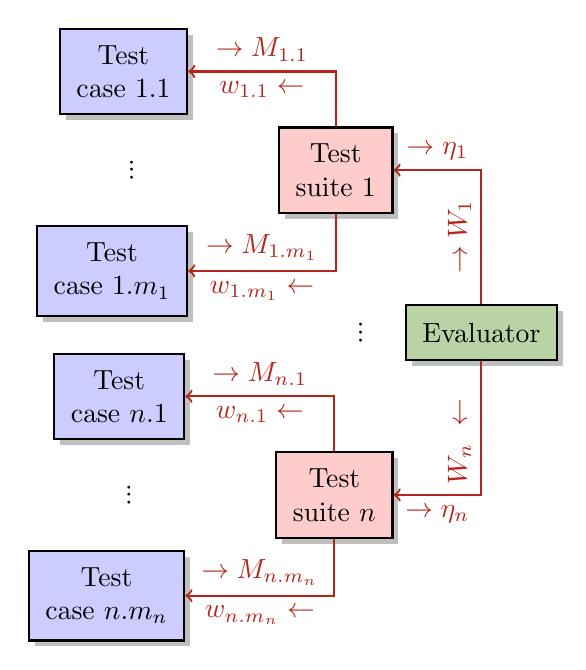
\begin{tikzpicture}
\node[bb](ev){Evaluator};

\node[bb, fill=Red!20, above left= 0.2cm of ev, yshift=1cm](ts1){Test \\ suite 1};
\draw[->, thick, BrickRed](ev) |- node[left, near start] {\rotatebox{90}{$\rightarrow W_1$}} node[above, near end] {$\rightarrow\eta_1$}(ts1);
\node[bb, fill=Red!20, below left= 0.2cm of ev, yshift=-1cm](tsn){Test \\ suite $n$};
\draw[->, thick, BrickRed](ev) |- node[above left] {\rotatebox{90}{$W_n\ \leftarrow $}} node[below, near end]{$\rightarrow\eta_n$}(tsn);

\node[bb, fill=Blue!20, above left= 0.2cm of ts1, xshift=-1cm](tc11){Test \\ case 1.1};
\draw[->, thick, BrickRed](ts1) |- node[below, near end] {$ w_{1.1} \leftarrow$} node[above, near end] {$\rightarrow M_{1.1}$}(tc11);

\node[inv, left= 1.5cm of ts1](dots2){\rotatebox{90}{...}};

\node[bb, fill=Blue!20, below left= 0.2cm of ts1, xshift=-1cm](tc1n){Test \\ case $1.m_1$};
\draw[->, thick, BrickRed](ts1) |- node[below, near end] {$w_{1.m_1} \leftarrow$} node[above, near end] {$\rightarrow M_{1.m_1}$} (tc1n);

\node[bb, fill=Blue!20, above left= 0.2cm of tsn, xshift=-1cm](tcm1){Test \\ case $n.1$};
\draw[->, thick, BrickRed](tsn) |- node[below, near end] {$ w_{n.1} \leftarrow$} node[above, near end] {$\rightarrow M_{n.1}$} (tcm1);

\node[inv, left= 1.5cm of tsn](dots3){\rotatebox{90}{...}};

\node[bb, fill=Blue!20, below left= 0.2cm of tsn, xshift=-1cm](tcmn){Test \\ case $n.m_n$};
\draw[->, thick, BrickRed](tsn) |- node[below, near end] {$w_{n.m_n} \leftarrow$} node[above, near end] {$\rightarrow M_{n.m_n}$} (tcmn);

\node[inv, left= 0.2cm of ev](dots4){\rotatebox{90}{...}};


\end{tikzpicture}
}

\end{center}
\caption{System Architecture}
\label{f:sarch}
\end{figure}

Figure ~\ref{f:sarch} shows the overall architecture under which the evaluation system works.

\subsection{Test cases}
For each programming problem, students typically write one program. Each question often has a number of testable aspects to be checked. In many many cases, these aspects roughly map to individual sub-questions; however, this is not necessary. Typically one, but sometimes more than one, test cases are created to check each of these testable aspects. Each test case is implemented as a function returning 1 on success and 0 on failure along with other relevant information.

\subsection{Test suites}
We would typically have a number of test cases to check a single problem. The number of test cases for question of average size is around 5-10. However, questions with up to 20-25 test cases are not uncommon. These test cases are then bundled into test suites. Hence, one test suite is created corresponding to each programming problem. A test suite computes an overall efficiency $\eta$, which is in the range 0 to 1, indicating the efficiency with which the corresponding problem was solved, corresponding to the problem under question by combining the result of all test cases. $\eta$ is computed as follows:

\begin{equation}
\eta = \frac{\Sigma wM}{\Sigma w}
\end{equation}

where $M$ is 1 or 0 depending on whether the corresponding test case passed or failed, and $w$ is the relative weight or importance of the aspect being tested by the corresponding test case.

\subsection{Evaluator}
All test suites are finally utilised by the central evaluator to compute the marks for the given problem as follows:
\begin{equation}
total = \Sigma \eta W
\end{equation}

where $W$ is the maximum marks allotted to the given problem.

 
\subsection{The Software}
The evaluation system for a specific assessment is a combination of assessment specific code written by the instructor/TA, and some boilerplate code already provided as part of the software. Instructor's main task is to create the individual test cases and place them under test suites. The boilerplate code provides the glue that puts together this code under the structure shown in fig.~\ref{f:sarch}. Additionally it provides utility scripts useful during the process of evaluation, e.g. preparing marks reports, sending emails, rudimentary plagiarism detection etc. The test case code written by the instructor, nevertheless, typically would run into several hundred lines of code. However, much of it is of repetitive nature. The system assists the instructor by generating stub code for such repetitive parts so that the instructor may focus on the assessment specific code.

In its current form, the system does not automatically design and generate test cases.

\section{Designing Questions}
An important objective of introductory programming courses is to introduce students to basic programming constructs (e.g. branches, loops, functions, recursion, classes and inheritance), and preliminary application of these to solve \emph{very simple} computing problems. These courses stop short of teaching more advanced program design concepts, e.g. data-structure and algorithm design, which are covered in later courses. This results in a fairly regimented nature of what can be asked and how these questions can be answered. The level of abstraction of questions focuses primarily on programming constructs and not on program design. For example, if a question is about implementation of the factorial function, it will mostly be specified if the solution should use iteration or recursion. Note that the objective of such a question would be to test whether the student has understood such programming concepts as loops or recursions, and not to test his/her understanding of the factorial function, which is either assumed to be known or is given in a mathematical form.

Questions designed at a high level of abstraction are desirable because they force the student to model the problem and design a solution. The number of design decisions the student has to take in this process commensurately increases the probability of going wrong or getting stuck. Succeeding in solving such a problem is a good indicator of the student having `got it'. However, not being able to solve such complex design problems is not an indicator that the student has not understood the concepts. In case of failure to solve a complex problem, the problem of analysing the exact reason for failure is often intractable, and totally not worth it.

The above observation allows designing questions at a very fine-grained level, without compromising what is being tested. Having said that, it is a significant challenge to design a question which does indeed test the student's knowledge on the topic in question. An obvious prerequisite to design such a question is a clarity about what is it that the student is supposed to know. Thus, questions should use \textit{learning objectives} as one of the primary references. If a learning objective requires the student to know how to write a for loop in Python, then any question that requires him/her to use for loop will suffice. For example:
\begin{enumerate}
\item Write a program that computes the factorial of a variable \lstinline@x@ which is defined in the beginning of the program. Use a for loop.
\item Write a program that prints "Hello world." ten times. Use a for loop.
\item Write a program that computes and prints the sum of all numbers in a list. Use a for loop.
\end{enumerate}

Note how some of the questions above are constraining the solution space to use only for loop. This is because the primary problem can be solved using other means too, e.g. while loop or recursion.

\section{Designing Test Cases}
From the point of view of test cases, there are a number of types of test cases each catering to a specific testing requirement. We elaborate on this aspect below.

\subsection{Programs with input/output} \label{s:pio}
If the output of the program is what needs to be tested, then the program should be executed and its output should captured appropriately to be compared against an expected output. This kind of programs are typically the first type of programs written by new programs.

\begin{mdframed}[frametitle=Example]
Write a program which takes two numbers as input representing the two
perpendicular sides of a right angled triangle, and prints out the length of the
hypotenuse.
\end{mdframed}

\begin{lstlisting}[style=pc]
@evaluate
def eval_1():
  subprocess.call(["cp", "drivers/Q1a_driver.py",
   "code/"])

  o = subprocess.check_output(["python",
       "code/Q1a_driver.py"])
  e = subprocess.check_output(["python",
      "mycode/Q1a_driver.py"])
  if(equals(o, e)):
    return (1, fname)
  else:
    return (0, fname + ": wrong answer")
\end{lstlisting}

The advantage with this kind of test cases is that they are by-and-large agnostic to the internal details of the program being evaluated. Hence, such test cases can be auto-generated to a large extent.

However, due to dependence on input/output (IO), such test cases also tend to be the most fragile: any mistake in the expected input format our the format of output results in the test case failing. Another common source of failure in this kind of test cases is spurious IO code inserted by the student during code, most probably for testing purpose, but later not removed during submission. This form of communication between the submitted program and test harness also puts severe limitations on the complexity or sophistication of the input/output data to/from the program.

There is no easy fix to the fragility of this form of test cases, nor are this kind of test cases entirely avoidable as, in most introductory programming courses, such problems must often be some of the first set of problems solved by the students.

%% TODO: Example
\subsection{Programs using/computing values}
Programs using input values from another part of the program computing values which then may get consumed by another part of the program are the next broad category of programs that students get to write. For example:

\begin{mdframed}[frametitle=Example]
Write a program to check if a given expression has balanced parentheses. The input string is allowed to contain only three types of brackets: parentheses, i.e. \lstinline[style=pc]@'('@/\lstinline[style=pc]@')'@, curly braces \lstinline[style=pc]@'{'@/\lstinline[style=pc]@'}'@ and square brackets \lstinline[style=pc]@'['@/\lstinline[style=pc]@']'@.

(Hint: Implement a stack in Python using lists)

\end{mdframed}

In the above problem, the student is required to accept the input in the form of a value stored in an input variable. Likewise, the solution program should store its result in an output variable.

The test case has to be designed to plug in input (program fragment that supplies input values to the submitted program) and output code (which traps the value generated by the submitted program and checks its correctness) to such programs. One way to do this is illustrated in the test case code written below. Here, the input values are present in input file \texttt{proginput.py}. The answer/result/output of the computation done by the student code is supposed to be stored in a variable named \lstinline[style=pc]|output| whose value is compared against the expected value (generated by the reference code). The advantage here is that the test case is agnostic to the internal details of the program under test, and hence, can by and large be auto-generated.

\begin{lstlisting}[style=pc]
def eval_program():
  subprocess.call(["rm", "mycode/proginput.py"])
  subprocess.call(["rm", "code/proginput.py"])
  subprocess.call(["cp", "input/proginput.py",
    "mycode/proginput.py"])
  subprocess.call(["cp", "input/proginput.py",
    "code/proginput.py"])
  import code.prog
  import mycode.prog

  if(equals(code.prog.output, mycode.prog.output)):
    return (1, "eval_prog" + ".eval_program")
  else:
    return (0, "eval_prog" +
     ".eval_program: wrong answer")
\end{lstlisting}


\subsection{Functions returning value}
The simplest and most robust type of test cases are those which test if the output returned by a particular function is correct or not, e.g. whether an implementation of factorial function indeed returns the correct value, or whether the area of a triangle is computed correctly based on its base and height. In most cases, the value returned from a function of this kind is a simple piece of data which can be directly compared with the expected value. Hence, the independence of the correctness of this kind of test (functions returning value) from any kind of interactive input/output makes them robust. The disadvantage of this kind of test cases also stems from the tight coupling between the test harness and the program under test, which makes it imperative that both be in the same programming language. Therefore, language independence is compromised.

\begin{mdframed}[frametitle=Example]
Implement a function that computes the factorial of a given number.
\end{mdframed}

\begin{lstlisting}[style=pc]
def eval_factorial():
  import code.factorial
  import mycode.factorial

  if(equals(code.factorial.factorial(5),
      mycode.factorial.factorial(5))):
    return (1, "eval_factorial" + ".eval_factorial")
  else:
    return (0, "eval_factorial" +
     ".eval_factorial: wrong answer")
\end{lstlisting}

\subsection{Functions with input/output}
There are function (procedures, to be precise) which depend on/result in \emph{side effects}, e.g. writing into the output console. Such functions should be called and their output (console) should captured appropriately.


\begin{mdframed}[frametitle=Example]
Implement a function that computes the factorial of a number input through standard input and prints out the result on the standard output.
\end{mdframed}

The test cases for such problems are similar to those involving direct input/output (section~\ref*{s:pio}). Hence, these test cases have a similar set of advantages and disadvantages as those. 

\subsection{Questions about Structural Properties}
This form of programming problems strictly do not test the functional properties of a program, but its structural aspects. We discuss this in more detail in a later section (section~\ref{s:tsa}).

\subsection{Between Robustness and Language Independence}

As is clear from the above types of test cases, there are two ideals which we aim to achieve in our test case design, and which are in apparent conflict with each other: \emph{robustness} on the one hand, and \emph{language independence} on the other. By robustness, we meet that the program under test and test harness communicate using rich data flow, involving complex data-structures if required. Language independence means that the implementation language of the test harness and that of the program under test need not be the same. This allows more code reuse on the side of the test harness and it is not required to re-implement the test harness for every new language used in the program under test.

If we wish to build robust test cases, we need to give more access for the test harness to the internals of the program under test. This mandates that they be written in the same language, thus compromising language independence. Contrariwise, if we wish to go for language independence, we have to decouple the test harness from the program under test. They limits the visibility that the test harness has into the internal data of the program under test. Result: they must communicate through some restricted channel like standard input/output. This precludes in memory data-flow between the two, hence impacting robustness negatively.

\section{Challenges with Testing Approach}
\subsection{Fragility}
There are several properties of a purely testing based approach of evaluation which present important challenges to implementing a robust and high-quality AEPA system through it. Some of these are pragmatic and lead to difficulties in designing a robust test harness itself. A representative set is given below:
\begin{enumerate}
\item \textbf{Crashes.} If the program under test runs as a part of the test harness program, a crash happening in the program under test may result in the whole test harness crashing. This could lead to the loss of all the results computing till the point of crash.
\item \textbf{Infinite loop.} In a similar manner, if the program under test gets stuck in an infinite loop, it blocks the whole testing process. Sometimes, the only way to come out of this stuck state is to abort the process, which again would lead to loss of work.

\end{enumerate}

These issues are well known in the software testing community, and as such can be solved using well known methods~\cite{Ammann:2008:IST:1355340}. For example, running the program under test as a separate process may safeguard the test harness process from crashing due to exceptions emerging from the program under test. Similarly, running the program under test as a separate thread with a timeout can be effective in preventing infinite loops to block the testing process indefinitely.


\subsection{Designing the oracle}
A more fundamental problem is that of designing the test oracle, again a well known problem to the testing community. In a majority of cases in introductory programming courses, verifying if the answer computed by the program under test is correct is easy. However, in many cases, this is not straightforward, especially when the result, instead of being a simple atomic piece of data, is a complex data structure. For example, comparing the equality of two sets is non-trivial, comparing the similarity (isomorphism) of two graphs is NP-hard, and comparing the semantic equivalence of two programs is undecidable. These difficulties may manifest themselves as test criteria depending on the assignment problem that the program is a solution to. The implementation of the oracle may turn out to be a very elaborate task, sometimes even impossible, in such cases. As mentioned earlier, in practice, such cases are not very prevalent. In may cases where they do occur, the problem can be bypassed by imposing constraints on the answer format to rule out difficult-to-manage variations between correct answers.

\section{Extensions to Testing Approach}
\subsection{Testing and Static Analysis} \label{s:tsa}
Some test cases may need to check static aspects of the program. Some of these can be dynamically checked through a cleverly designed test case. However, in general, such features are not open to be tested dynamically, but have to be checked by performing static analysis\cite{Aho:2006:CPT:1177220} of the source code.

\begin{mdframed}[frametitle=Example 1]
Implement the factorial function using recursion.
\end{mdframed}

This is an example of a case which is not in principle amenable to purely testing based evaluation, but can be handled using a trick. In this example, a factorial function written using loops (incorrect solution) will produce identical results as one implemented using recursion (correct solution). Hence, normal test cases will not be able to detect that a loop-based solution is not the correct solution. However, a clever trick can be used to detect presence of recursion -- by using stack overflow. In most programming languages, deeper recursions will lead to a proportional growth of the depth of the program stack. A sufficiently deep recursion will lead to the program stack to overflow. This can be utilised to detect if a the implementation indeed uses recursion. However, there are programming languages in which functions can be implemented that can go up to arbitrary depths of recursion without overflowing the stack. The given trick will fail in the case of such programming languages.

\begin{mdframed}[frametitle=Example 2]
Design two classes \lstinline[style=pc]|A| and \lstinline[style=pc]|B| such that \lstinline[style=pc]|B| is a subclass of \lstinline[style=pc]|A|. Give \lstinline[style=pc]|A| a method \lstinline[style=pc]|m|. Instantiate \lstinline[style=pc]|B| as \lstinline[style=pc]|b|, and call \lstinline[style=pc]|m| on \lstinline[style=pc]|b|. 
\end{mdframed}

The point of the above problem is to check if the student is aware that it is possible to call a method of a super-class through an instance of a subclass. The expectation is that a student who knows this fact will not give any method \lstinline[style=pc]|m| to class \lstinline[style=pc]|B| knowing that \lstinline[style=pc]|A.m| is callable from an instance \lstinline[style=pc]|B|. This is an example of a case where testing based method will not work at all. Here, if we instantiate an object \lstinline@b@ of class \lstinline@B@, and call \lstinline@b.m@, there is no way to tell by observing the output of the program if the method \lstinline@m@ is a member of class \lstinline@A@ (correct solution) or of \lstinline@B@ (incorrect solution). Thus, in general, pure testing based approach fails to deal with this scenario.

A workaround is possible depending on the specific implementation programming language.

The above code shows a test case that checks (at runtime) if the method \lstinline@m@ is member of class \lstinline@B@, which is static/structural feature of the program under test. The programming language is Python and the feature used to enable implementation of this test is called \emph{reflection}. Reflection is a feature provided by certain programming languages that allows the program to inspect its own structure at runtime. Whether such a test case can be implemented or not for check for a structural property depends on whether and to what extent the programming language provides reflection.


\subsection{Static Analysis} \label{s:aepa1}
In situations where the competency under evaluation translates to a structural aspect of the program under evaluation, the presented approach would no more be effective in its present form, particularly when the programming language in question does not have features like reflection. This is where the evaluation system must have built into it a language front-end that parses the program under evaluation and creates an internal representation of the same, e.g. an abstract syntax tree, that can then be analysed by a static analysis procedure.

\begin{figure}

\begin{center}
\resizebox{\textwidth}{!}{
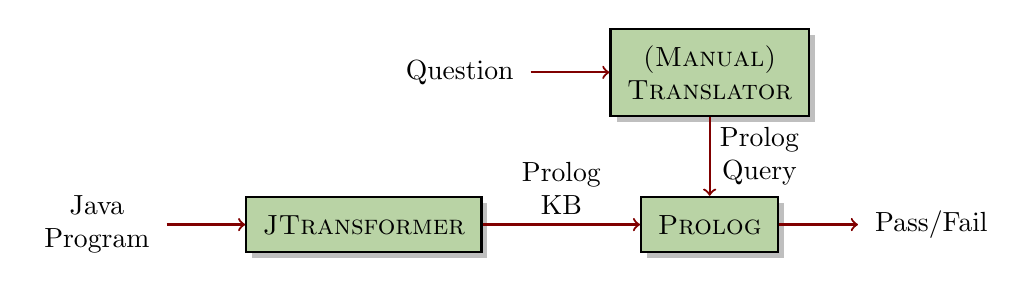
\begin{tikzpicture}
\node[inv] (inp) {Java \\ Program};
\node[bb, right = of inp] (fe){\textsc{JTransformer}};
\node[bb, right = 2cm of fe] (ver) {\textsc{Prolog}};
\node[bb, above = of ver] (xr) {\textsc{(Manual)} \\ \textsc{Translator}};
\node[inv, left = of xr] (q) {Question};
\node[inv, right = of ver] (res) {Pass/Fail};

\draw[->, thick, draw=Maroon] (inp) to (fe);
\draw[->, thick, draw=Maroon] (fe) to node[above, align=center]{Prolog \\ KB}(ver); 
\draw[->, thick, draw=Maroon] (xr) to node[right, align=center]{Prolog \\ Query}(ver); 
\draw[->, thick, draw=Maroon] (ver) to (res); 
\draw[->, thick, draw=Maroon] (q) to (xr); 

\end{tikzpicture}
}
\end{center}
\caption{Static Analysis: An evaluation system based on static analysis using Prolog}
\label{f:jtsa}
\end{figure}

Figure~\ref{f:jtsa} presents a scheme that we have devised to do static analysis based AEPA of Java programs. The program under evaluation is parsed and converted into a Prolog fact base by an off-the-shelf front-end tool called JTransformer. The question is posed as a Prolog query which evaluates if the program structure satisfies the property under question. Given below is a Prolog query to check if a function is recursive or not.

\begin{lstlisting}[style=pc]
findrecursiveMethod(MethodName) :-   
    methodT(MethodT_1,ClassT,MethodName,
      [ParamT_1],BasicTypeT,[],[],BlockT_1)
  ,	paramT(ParamT_1,MethodT_1,BasicTypeT_1,i), 
  	  blockT(BlockT_1,MethodT_1,MethodT_1,
  	  [ExecT_1])
  ,	execT(ExecT_1,BlockT_1,MethodT_1,CallT_1)
  ,	callT(CallT_1,ExecT_1,MethodT_1,null,
      [LiteralT_1],MethodT_1,[],BasicTypeT)
  ,	literalT(LiteralT_1,CallT_1,MethodT_1,
      BasicTypeT_1,'0').
\end{lstlisting}

We are currently working on extending this idea to other programming languages. Each programming language requires a separate front-end in place.

\subsection{Static Analysis and Machine Learning} \label{s:aepa2}
The objective of evaluation is to test some aspect of student knowledge on a specific topic. However, due to a variety of reasons, the translation of the student's knowledge into a correct answer to an exam question has several hurdles. Consequently, a student may often make mistakes while writing a program which may cause the program to fail all test cases, or may lead to an internal representation which a traditional algorithm would judge as structurally unrelated to the correct solution.

Presented below is a Python code for computing the transpose of a matrix. Interestingly, if the instruction \lstinline[style=pc]@n.append(row)@ is written with two extra leading spaces, it will push the instruction into the for loop, completely changing the meaning of the program.
\begin{lstlisting}[style=pc]
m = [  [1, 2, 3],  [4, 5, 6] ]
n = []
for i in range(len(m[0])):
  row = []
  for j in range(len(m)):
    row.append(m[j][i])
  n.append(row)
print n
\end{lstlisting}

Another reason why an exhaustive static analysis based approach may not work is because of its computational cost. In large classes with thousands of submissions, the high computational cost of doing elaborate static analysis may be completely unscalable.

In such situations, the AEPA approach must go beyond strict static analysis which does an exact analysis looking for presence or absence of a particular feature. There should be scope for approximate analysis that identifies and gives credit to broad similarity with some reference solution.

\begin{figure}

\resizebox{\textwidth}{!} {
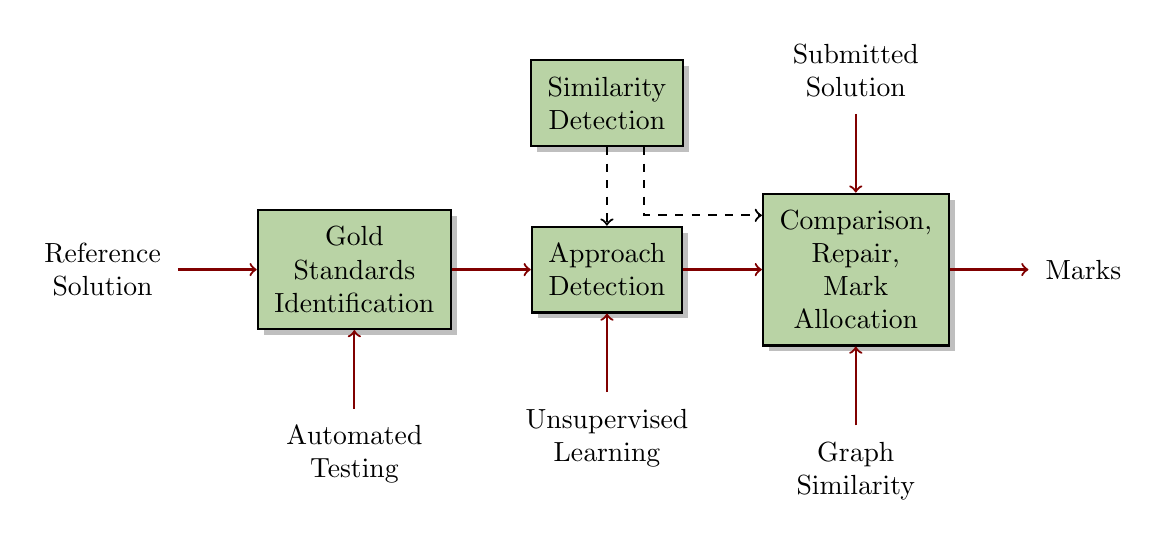
\begin{tikzpicture}
    \node[inv] (1)  {Reference \\ Solution};
    \node[bb]  (2) [right = of 1]   {Gold \\ Standards \\ Identification};
    \node[bb]  (3) [right = of 2]   {Approach \\ Detection};
    \node[bb] (4) [right = of 3] {Comparison, \\ Repair, \\ Mark \\ Allocation};
    \node[inv] (5) [above = of 4] {Submitted \\ Solution};
    \node[inv] (6) [right = of 4] {Marks};
    \node[bb] (simdet) [above = of 3] {Similarity \\ Detection};

    \node[inv,outer sep=0] (2a) [below = of 2] {Automated \\ Testing};
    \node[inv,outer sep=0] (3a) [below = of 3]   {Unsupervised \\ Learning};
    \node[inv,outer sep=0] (4a) [below = of 4] {Graph \\ Similarity};

	\draw[->, thick, draw=Maroon] (1) -- (2);
	\draw[->, thick, draw=Maroon] (2) -- (3);
	\draw[->, thick, draw=Maroon] (3) -- (4);
	\draw[->, thick, draw=Maroon] (4) -- (6);
	\draw[->, thick, draw=Maroon] (5) -- (4);

	\draw[->, thick, dashed] (simdet) -- (3);
	\draw[->, thick, dashed] (simdet.310) |- (4.150);

	\draw[->, thick, draw=Maroon] (2a) -- (2);
	\draw[->, thick, draw=Maroon] (3a) -- (3);
	\draw[->, thick, draw=Maroon] (4a) -- (4);

  \end{tikzpicture}
}
\caption{An AEPA Approach using Machine Learning}
\label{f:aepaml}
\end{figure}

Various approaches have been explored for automated evaluation of programming assignments, e.g. machine learning\citet{Singh:2016:QIG:2939672.2939696,Srikant:2014:SGC:2623330.2623377}, finite state machines\citet{Sharma:2014:SAE:2662117.2662127}, program synthesis\citet{DBLP:conf/cav/DAntoniSS16}.

Figure~\ref{f:aepaml} shows an approach we have devised (work in process) that uses a combination of testing, static analysis and machine learning to automatically evaluate programming assignments. The details of this work are outside the scope of this paper, but we present an overview of the approach below.

In this approach, we essentially award marks to an answer program partly based on some measure of similarity of a submitted code to some model answer. Our AEPA approach consists of the following top-level modules:
\begin{itemize}
\item \textbf{Gold standard identification.} The first module segregates all the submitted programs into those which pass all the test cases, and those which do not pass on all the test cases. The former category is called the \emph{gold standard solution}.

\item \textbf{Similarity estimation.} The second module is responsible for quantifying the structural similarity between two given program. 
\item \textbf{Approach detection.} In large classes, students often come up with creative approaches to solve a problem which the instructor may not be able to enumerate or foresee. Approach detection module employs techniques from unsupervised machine learning to detect the solution approaches used by all submissions. Similarity estimation builds on significant work done in this area of plagiarism detection \cite{Liu,Schleimer,Sajnani}.


\item \textbf{Marking.} The final module uses a machine learning model trained using a ground truth data obtained from manual grading done on a training data-set to give marks to the submitted solutions. In this module, we use both structural similarity and test results for training the model.
\end{itemize} 

\section{Experience}
The AEPA system described in this paper has been used as a part of an introductory programming course (Programming - Python) and an advanced course on Programming Languages that the author teaches at his university. Though no formal data collection has been made, following are some rough figures:
\begin{enumerate}
\item \textbf{Evaluation scale.} Each run of a course typically has 7-8 programming assignments. Each assignment has 5-10 programming questions, each in turn having 2-5 sub questions. Further, there are two large examinations conducted, each of a scale of a single assignment sheet.
\item \textbf{Program size.} Each question involves at the minimum writing minimum of 2-3 lines of code and maximum of 25-30 lines of code.
\item \textbf{Assessment effort.} The class size is about 120 students. This gives us an estimated 18000-20000 programming questions to be evaluated over the semester. Even with a minute spent manually evaluating each question (which is a conservative estimate), the evaluation effort over the entire semester is about 40 days excluding other non-programmatic assessments (theory, project demos etc.). Considering a semester with about 90-100 working days in it, this amounts to close to nearly half the entire duration of the semester. This is clearly far above what an instructor can afford to spend on evaluating answers. Even if some of this work is offloaded to TAs (which is not an easy thing to do in our circumstances), the high cost of the evaluation process can not be ignored.
\end{enumerate}

Contrary the manual evaluation, the author has been able to do all corrections automatically with no or very little help from the TAs using the system presented in this paper. The major portion of the effort in this approach goes in designing the questions and test cases. Each assessment instrument (assignment/examination) requires about one day's effort to create the questions and test cases. Automated evaluation requires about 1-2 hours' effort. Detailed evaluation reports get prepared and sent to the students immediately after the evaluation gets done. This significantly shortens the feedback cycle length. Though we do not yet have enough longitudinal data, it is expected that the evaluation effort will drop significantly in future when it gets amortised over all the times an item already added to the item bank is reused.

Following are the achievements of our approach to automated evaluation. Some of these are advantages with respect to platforms like DomJudge:
\begin{enumerate}
\item \textbf{Simple setup.} Our system is based on the policy of having all data on the local machine. This simplifies the setup of the system which is lightweight and local. The boilerplate library code is all in Python. Hence, software requirements are very minimal and light.
\item \textbf{Simple use.} Likewise, the actual evaluation also happens on the local machine of the instructor/TA. No connection to the Internet is required. Of course, a learning management system like \cite{moodle} may be used to facilitate release of the assignment and submissions, but is not essential.
\item \textbf{Language independence.} It is straightforward to use the AEPA system for assignments in a variety of programming languages as the test cases can be designed to be language independent.
\item \textbf{Data availability.} As the code submitted is not locked inside the database of the system, extracting them for any other purpose is not an issue at all. The code that was submitted for evaluation using our system during our courses have been extensively used by us for our other related research work (see sections \ref{s:aepa1} and \ref{s:aepa2}).
\end{enumerate}

\section{Conclusion}
In this paper, we have described a homegrown AEPA system. We have defined an overall architecture of evaluation. We have identified the parts of automated evaluation which are repeatable across assessments; such parts are extracted into boilerplate modules of our system. The rest of the part is assessment specific which must be coded out by the evaluator based on the specific needs of the assessment. We have explained the process involved in writing test cases, based on a set of test case types identified here.


Automated evaluation is a holy grail of pedagogy which has the potential of allowing great scale up and boost to quality of teaching and learning by freeing up enormous amount of time for instructors which currently gets wasted unproductively in marking answers. Automated evaluation at scale of all types of answers (e.g. essay type, mathematical models and proofs etc.) are well out of the reach of the current day technology (though research is ongoing in all these areas). Automated evaluation of programming assignments is the first frontier of success of this technology. As a practical problem, there exist numerous solutions including the one described here. All these approaches take a purely testing based. Testing based approaches have their own limitation, both of practical and fundamental nature. We have noted these challenges in this testing based approach. Advanced approaches to automated evaluation that try to overcome these challenges are an area of active research. We have outlined two of our current research projects which are aimed at tackling these challenges: one based on pure static analysis, and the other based on a combination of testing, static analysis and machine learning.

Our future research has two main aims: one, to make fundamental contributions to the algorithmic issues involved in the AEPA problem; two, to improve the current system to offer better functional and usability features: e.g. web-based/GUI interface, automated test generation, and more fine-grained characterisation of question and test case types. 

\bibliography{references}
\bibliographystyle{apalike}

\section{A Detailed Example}

\begin{mdframed}[frametitle=Example]
Implement a class named \lstinline[style=pc]|BankAccount| with the following features:
\begin{enumerate}
\item Attribute \lstinline[style=pc]|balance| that reflects the current balance in the account.
\item A constructor that allows instantiating a \lstinline[style=pc]|BankAccount| object with an explicit initial \lstinline[style=pc]|balance| amount. If this is not provided, the default amount is set to 0. For example:
\begin{lstlisting}[style=oc]
>>> a1 = BankAccount(100)
>>> a1.balance
100
>>> a2 = BankAccount(0)
>>> a2.balance
0
\end{lstlisting}
\end{enumerate}
\end{mdframed}

The above problem has several testable aspects. As mentioned above, some of them derive directly from the way the question is phrased, while some have to be derived. Here are some of these aspects:

Is the student able to:
\begin{enumerate}
\item define a class in the given programming language?
\item add an attribute to a class?
\item define a constructor and use it to initialise an attribute?
\item use the constructor to initialise an attribute with a default value?
\end{enumerate}

As is expected, each of the above question would give rise to at least one test case, and it turns out that way. Some test cases are presented below:
\begin{lstlisting}[style=pc]
# Test objective:
# * define a class 
# * define a constructor and use it to initialise an 
#    attribute
@evaluate
def eval_1():
  import code.bank1
  a = code.bank1.BankAccount(20)
  return (1, "eval_bank1.eval_1")

# Test objective:
#  * define a constructor and use it to initialise an
#    attribute
@evaluate
def eval_2():
  import code.bank1
  a = code.bank1.BankAccount(20)
  if(equals(a.balance, 20)):
    return (1, "eval_bank1.eval_2")
  else:
    return (0, "eval_bank1.eval_2: wrong answer")

# Test objective: 
# * use the constructor to initialise an attribute with
#   a default value
@evaluate
def eval_3():
  import code.bank1
  a = code.bank1.BankAccount()
  if(equals(a.balance, 0)):
    return (1, "eval_bank1.eval_3")
  else:
    return (0, "eval_bank1.eval_3: wrong answer")
\end{lstlisting}


\end{document}